% This is text associated with the open textbook "Open Electromagnetics"
% See immediately below for author, date
% This work is licensed under the Creative Commons Attribution-ShareAlike 4.0 International License. (CC BY-SA 4.0) 
% To view a copy of the license, visit http://creativecommons.org/licenses/by-sa/4.0/

%ORB TITLE Input Impedance of a Terminated Lossless Transmission Line
%ORB AUTHOR 0        # S.W. Ellingson, Virginia Tech (ellingson@vt.edu)
%ORB DATE 20180802   # yyyymmdd
%ORB ABSTRACT Input Impedance of a Terminated Lossless Transmission Line 

\label{m0087_Input_Impedance_of_a_Terminated_Lossless_Transmission_Line} % <-- Must match name of this file and module directory name.  Don't mess with this!
\index{transmission line!input impedance|(}

Consider Figure~\ref{m0087_fZinTerminatedTL}, which shows a lossless transmission line being driven from the left and which is terminated by an impedance $Z_L$ on the right.
If $Z_L$ is equal to the characteristic impedance  $Z_0$ of the transmission line, then the input impedance $Z_{in}$ will be equal to $Z_L$.
Otherwise $Z_{in}$ depends on both $Z_L$ and the characteristics of the transmission line. 
In this section, we determine a general expression for $Z_{in}$ in terms of $Z_L$, $Z_0$, the phase propagation constant $\beta$, and the length $l$ of the line. 
%
\begin{figure}[b!]
\begin{center}
\pdftooltip{{  % note double brace
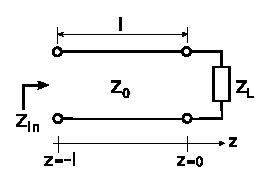
\includegraphics[width=2in]{modules/m0087_fZinTerminatedTL.eps}
}}{A transmission line with two nodes on both the input and output branches. The input node is open and the output node has an impedance labeled Z sub L. Starting at the top left and going clockwise, l is measured between the source terminal and the load terminal. The output of the load is measured at z=0, and the source is at z equal to -l. }
\end{center} 
\caption{\label{m0087_fZinTerminatedTL}A transmission line driven by a source on the left and terminated by an impedance $Z_L$ at $z=0$ on the right.}
\end{figure}   
 
Using the coordinate system indicated in Figure~\ref{m0087_fZinTerminatedTL}, the interface between source and transmission line is located at $z=-l$.  
Impedance 
is defined at the ratio of potential to current, so: 
%
\begin{equation}
Z_{in}(l) \triangleq \frac{\widetilde{V}(z=-l)}{\widetilde{I}(z=-l)} 
\end{equation}
%
Now employing expressions for $\widetilde{V}(z)$ and  $\widetilde{I}(z)$ from Section~\ref{m0086_Standing_Waves} with $z=-l$, we find:
%
\begin{flalign}
Z_{in}(l) &= \frac{V_0^+ \left( e^{+j\beta l} + \Gamma e^{-j\beta l} \right)}{V_0^+ \left( e^{+j\beta l} - \Gamma e^{-j\beta l} \right)/Z_0} \nonumber \\
          &= Z_0 \frac{ e^{+j\beta l} + \Gamma e^{-j\beta l} }{ e^{+j\beta l} - \Gamma e^{-j\beta l} }
\end{flalign}
%
Multiplying both numerator and denominator by $e^{-j\beta l}$:
%
\begin{equation}
\boxed{
Z_{in}(l) = Z_0 \frac{ 1 + \Gamma e^{-j2\beta l} }{  1 - \Gamma e^{-j2\beta l} }
}
\label{m0087_eZin1}
\end{equation}
%
Recall that $\Gamma$ in the above expression is:
%
\begin{equation}
\Gamma = \frac{ Z_L-Z_0 }{  Z_L+Z_0}
\label{m0087_eGamma}
\end{equation}

Summarizing:
%
%ORB HIGHLIGHT
\begin{mdframed}[backgroundcolor=yellow!20,nobreak=true]
Equation~\ref{m0087_eZin1} is the input impedance of a lossless transmission line having characteristic impedance $Z_0$ and which is terminated into a load $Z_L$.  The result also depends on the length and phase propagation constant of the line. 
\end{mdframed}
%
%TODO: PROBLEM: {\color{red}(PROBLEM: SHOW $Z_{in}(l=0)=Z_L$.)}

Note that $Z_{in}(l)$ is periodic in $l$.
Since the argument of the complex exponential factors is $2\beta l$, the frequency at which $Z_{in}(l)$ varies is $\beta/\pi$; and since $\beta=2\pi/\lambda$, the associated period is $\lambda/2$.  
This is very useful to keep in mind because it means that all possible values of $Z_{in}(l)$ are achieved by varying $l$ over $\lambda/2$.  
In other words, changing $l$ by more than $\lambda/2$ results in an impedance which could have been obtained by a smaller change in $l$.
Summarizing to underscore this important idea:
%
%ORB HIGHLIGHT
\begin{mdframed}[backgroundcolor=yellow!20,nobreak=true]
The input impedance of a terminated lossless transmission line is periodic in the length of the transmission line, with period $\lambda/2$.
\end{mdframed}

Not surprisingly, $\lambda/2$ is also the period of the standing wave (Section~\ref{m0086_Standing_Waves}).
This is because -- once again -- the variation with length is due to the interference of incident and reflected waves.

Also worth noting is that Equation~\ref{m0087_eZin1} can be written entirely in terms of $Z_L$ and $Z_0$, since $\Gamma$ depends only on these two parameters.  
Here's that version of the expression:
%
\begin{equation}
Z_{in}(l) = Z_0 \left[ \frac{ Z_L + jZ_0\tan\beta l }{ Z_0 + jZ_L\tan\beta l } \right]
\label{m0087_eZin2}
\end{equation}
%
This expression can be derived by substituting Equation~\ref{m0087_eGamma} into Equation~\ref{m0087_eZin1} and is left as an exercise for the student.
%
%TODO PROBLEM: {\color{red}(PROBLEM: DERIVE ABOVE EQUATION)}

Finally, note that the argument $\beta l$ appearing Equations~\ref{m0087_eZin1} and \ref{m0087_eZin2} has units of radians and is referred to as \emph{electrical length}.
\index{electrical length}
Electrical length can be interpreted as physical length expressed with respect to wavelength and has the advantage that analysis can be made independent of frequency.  

\index{transmission line!input impedance|)}
